\scanpage{8}
\figure{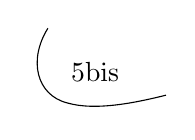
\begin{tikzpicture}[x=1cm,y=1cm]
\node at (.7,.45) {\mspage{5bis}};
\draw (.1,1.0) .. controls (-.15,.6) and (-.05,.15) .. (.35,.05) .. controls (.7,-.05) and (1.2,.05) .. (1.6,.15);
\end{tikzpicture}}
5. On peut aussi donner une condition d'\uline{existence} des $\pi_i$, liée aux conditions $(4.4)$. Pour ceci, on suppose que $\mathcal E$ est contenu dans un sur-anneau gradué $\mathcal F$ [p.ex. \inserted{\figure{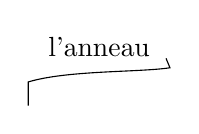
\begin{tikzpicture}[x=1cm,y=1cm,baseline=(reading.base)]\node (reading) at (0,.35) {l'anneau};\draw (-.9,-.4)--(-.9,-.1) .. controls (-.4,.05) and (.5,.02) .. (.9,.08)--(.85,.2);\end{tikzpicture}}} des endom. d'un $M^*$ comme dans 1.] pour lequel les $\pi_i$ satisfont $(1.1.)$ et les relations correspondantes à $(1.3)$ (avec $\mathcal E$ remplacé par $\mathcal F$) sont satisfaites; \inserted{\figure{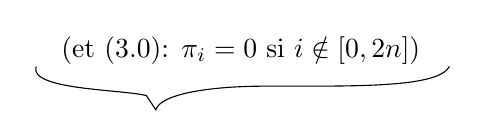
\begin{tikzpicture}[x=1cm,y=1cm,baseline=(reading.base)]\node (reading) at (0,.35) {(et $(3.0)$: $\pi_i=0$ si $i\notin[0,2n]$)};\draw (-2.6,.15) .. controls (-2.7,-.15) and (-1.5,-.14) .. (-1.2,-.22)--(-1.08,-.4) .. controls (-1.02,-.2) and (-.4,-.1) .. (.3,-.1) .. controls (1.5,-.1) and (2.5,-.12) .. (2.65,.15);\end{tikzpicture}}} Supposons que $\forall i$, la condition $(4.4)_i$ soit satisfaite, (avec $v_i,w_i\in\mathcal E$ bien sûr). On va en conclure que
\[
\pi_i\in\mathcal E\quad\text{pour tt }i.
\tag{5.1}
\]
\deleted{\unsure{Raisonnons par récurrence sur $i$.}}\inserted{Supposons prouvé \deleted{que} déjà $\pi_\alpha\in\mathcal E$ si $\alpha\notin[i,2n-i]$,} où $i<n$, et prouvons que l'on peut remplacer $i$ par $i+1$, \inserted{\figure{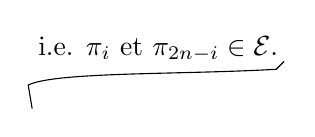
\begin{tikzpicture}[x=1cm,y=1cm,baseline=(reading.base)]\node (reading) at (0,.35) {i.e. $\pi_i$ et $\pi_{2n-i}\in\mathcal E$.};\draw (-1.6,-.4)--(-1.65,-.1) .. controls (-1.3,.07) and (.3,.03) .. (1.5,.1)--(1.6,.2);\end{tikzpicture}}}\inserted{Trivial si $i=n-1$, supposons que $i\leq n-2$.}

Notons que, avec les notations de 3., \deleted{\unsure{on a}}\inserted{\figure{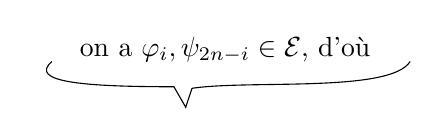
\begin{tikzpicture}[x=1cm,y=1cm,baseline=(reading.base)]\node (reading) at (0,.35) {on a $\varphi_i,\psi_{2n-i}\in\mathcal E$, d'où};\draw (-2.2,.2) .. controls (-2.5,-.06) and (-1.8,-.12) .. (-.65,-.12)--(-.5,-.38)--(-.42,-.14) .. controls (.3,-.03) and (2.1,-.2) .. (2.35,.2);\end{tikzpicture}}} \deleted{\unsure{remplaçons} $v_i,\inserted{w_i}$ par} \deleted{\unsure{alors}}\inserted{donc} $\psi_{2n-i}v_i\varphi_i$, $\varphi_iw_i\psi_{2n-i}\in\mathcal E$, i.e.
\[
\left\{\begin{aligned}
\inserted{v'_i={}}\psi_{2n-i}v_i\varphi_i&=\pi_{2n-i}v_i\pi_i\in\mathcal E\\
\inserted{w'_i={}}\varphi_iw_i\psi_{2n-i}&=\pi_iw_i\pi_{2n-i}\in\mathcal E
\end{aligned}\right.
\]
et \uline{co}mme \deleted{donc}
\[
w'_iv'_i=\pi_iw_i\pi_{2n-i}v_i\pi_i
\inserted{\text{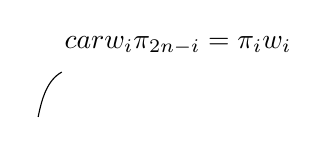
\begin{tikzpicture}[x=1cm,y=1cm,baseline=(reading.base)]\node (reading) at (0,.35) {$\quad\text{car }w_i\pi_{2n-i}=\pi_iw_i$};\draw (-1.6,-.55) .. controls (-1.55,-.3) and (-1.48,-.08) .. (-1.3,.02);\end{tikzpicture}}}\]
\[
=\pi_i\pi_iw_iv_i\pi_i
\inserted{\text{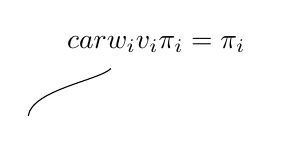
\begin{tikzpicture}[x=1cm,y=1cm,baseline=(reading.base)]\node (reading) at (0,.35) {$\quad\text{car }w_iv_i\pi_i=\pi_i$};\draw (-1.45,-.55) .. controls (-1.4,-.22) and (-.55,-.1) .. (-.4,.05);\end{tikzpicture}}}
=\pi_i^3=\pi_i.
\]
et de $=$ \deleted{$\unsure{=\pi_i}$} $v'_iw'_i=\pi_{2n-i}$, on conclut que $\pi_i\in\mathcal E$, $\pi_{2n-i}\in\mathcal E$.
\mspage{7}
